\chapter*{Annexes}
\addcontentsline{toc}{chapter}{Annexes}
%Le lecteur n'est pas obligé de les lire pour évaluer votre travail. Il s'agit d'un complément auquel pourrait se reporter le lecteur.
%Par exemple, vous pourriez mettre une copie d'écran, un extrait de code, etc. Gardez à l'esprit que le lecteur devrait comprendre le rapport sans se reporter aux annexes. Si ce n'est pas le cas, alors l'information devrait apparaître dans le corps du rapport et non en annexe.
%Dans tous les cas, les annexes doivent être citées dans le corps du rapport. Par exemple: "(cf. annexe XX)" ou "Pour plus de détails, le lecteur pourra se reporter à l'annexe XX page XX."

\subsection*{Annexe I - Cycle de développement (en V) }

%\begin{center}
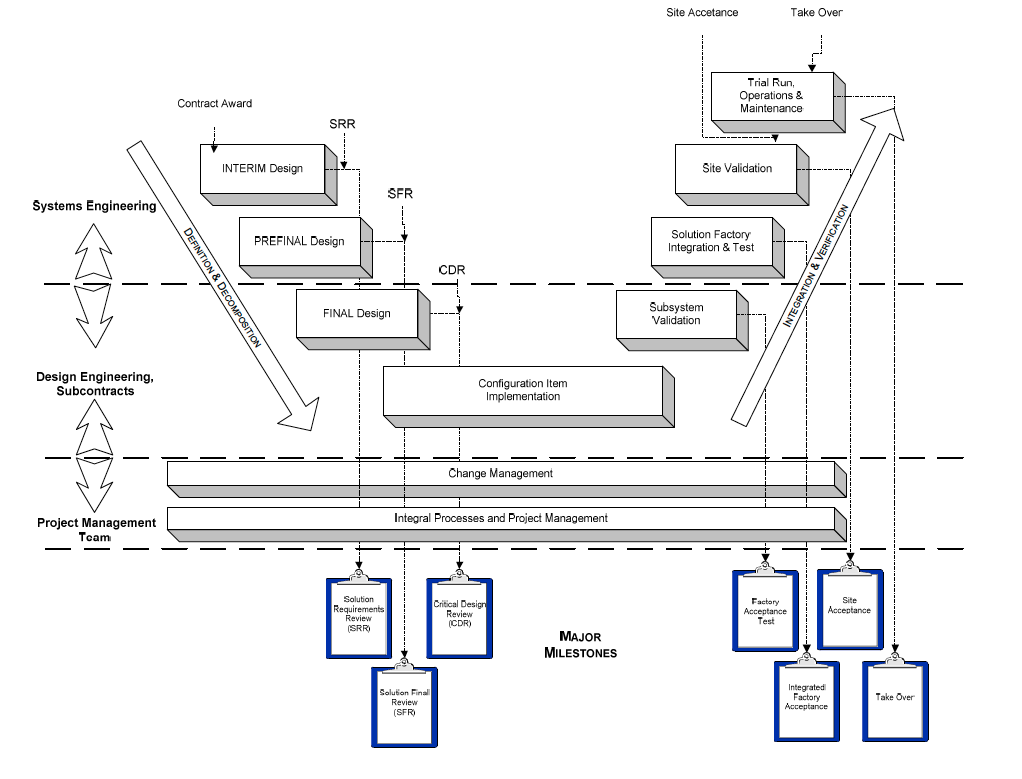
\includegraphics[height=14cm]{ressources/images/annexes/Vcycle.png}
%\end{center}

\subsection*{Annexe II - Extrait de la convention de nommage }

\begin{center}
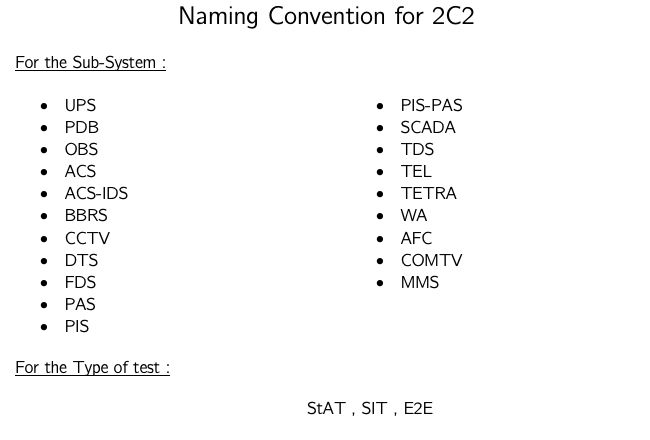
\includegraphics[scale=0.75]{ressources/images/annexes/convention.png}
\end{center}
